% Independent matrix anchors and TeX hboxes, in TeX points.
\documentclass{article}
\usepackage{pgfplots}
\usetikzlibrary{plotmarks}
\pgfplotsset{compat=1.18}
\newcommand{\ptat}[2]{\pgfextractx{\dimen0}{\pgfpointanchor{#1}{#2}}%
  \pgfextracty{\dimen2}{\pgfpointanchor{#1}{#2}}\typeout{POINT #1.#2 \the\dimen0,\the\dimen2}}
\newcommand{\sample}[2]{\draw[#2,mark repeat=2,mark phase=2] plot coordinates
  {(0cm,0cm)(.3cm,0cm)(.6cm,0cm)};\coordinate[overlay] (#1) at (.3,0);}
\newcommand{\report}{\ptat{L}{north west}\ptat{L}{south east}
  \ptat{S1}{center}\ptat{S2}{center}\ptat{T1}{text}\ptat{T2}{text}}
\begin{document}
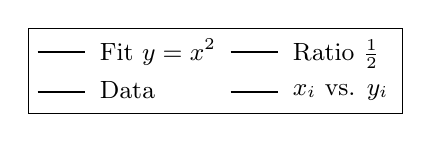
\begin{tikzpicture}
  \matrix[/pgfplots/every axis legend,anchor=north,font=\small,
    cells={anchor=west},column sep=3pt,row sep=2pt] (L) {
    \sample{S1}{thick} & \node(T1){Fit $y=x^2$}; &
    \sample{S2}{thick} & \node(T2){Ratio $\frac{1}{2}$};\\
    \sample{S3}{thick} & \node(T3){Data}; &
    \sample{S4}{thick} & \node(T4){$x_i$ vs. $y_i$};\\};
  \report\ptat{T3}{text}\ptat{T4}{text}
\end{tikzpicture}
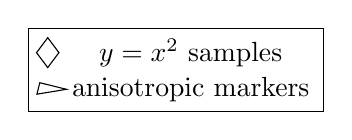
\begin{tikzpicture}
  \matrix[/pgfplots/every axis legend,anchor=north] (L) {
    \sample{S1}{only marks,mark=diamond*,mark size=4pt,mark options={scale=1.35}}
      & \node(T1){$y=x^2$ samples};\\
    \sample{S2}{only marks,mark=triangle*,mark size=4pt,mark options={xscale=1.7,yscale=.6,rotate=25}}
      & \node(T2){anisotropic markers};\\};
  \report
\end{tikzpicture}
\end{document}
